\documentclass[a4paper,10pt,twoside]{article}

% Note that if you want to use the \begin{equation} ... \end{equation}
% environment, you will have to include fleqn in the
% \documentclass[...]{...} options! 
% The top of your LaTeX file should then look like this:
% \documentclass[a4paper,10pt,twoside,fleqn]{article}

\usepackage{clin}        % Stylefile for CLIN Journal
\usepackage{harvard}     % Bibliography Stylefile
%\usepackage{...,cgloss4e,avm,trees,tree-dvips,gb4e,ipa,graphicx}
                         % Whatever other packages you need
% Harvard:
% \cite{Covington}             (Covington 1994)
% \citeasnoun{Covington}       Covington (1994)
% \citeyear{Covington}         (1994)


%tikz packages for drawing grammar trees
\usepackage{tikz}
\usepackage{tikz-qtree}
\usetikzlibrary{positioning}

\usepackage{amsmath,amssymb}

\pagestyle{empty}

\begin{document}

\title{Neural processing of sentences}

\author{Amelia Burroughs$^*$ \email{amelia.burroughs@bristol.ac.uk}\\
{\normalsize \bf Nina Kazanina}$^{**}$ \email{nina.kazanina@bristol.ac.uk}\\
{\normalsize \bf Conor Houghton}$^*$ \email{conor.houghton@bristol.ac.uk}
\AND \addr{$^*$Department of Computer Science, University of Bristol, UK}
\AND \addr{$^{**}$School of Psychological Science, University of Bristol, UK} }


\maketitle\thispagestyle{empty} % extra pagestyle command for first page

\begin{abstract}

How the human cognitive system is able to comprehend language has been
a matter of recent debate. On the one hand the brain may make use of
learned grammatical rules to decompose sentences into a hierarchy of
syntactic structures to generate meaning. On the other hand the brain
may rely on simpler, statistical methods where the generation of
meaning relies on sequentia processing of lexical information. To
investigate these we recorded EEG from participants as they listen to
streams of isochronously-presented words. In our different conditions
there are grammatical and semantic manipulationa: the words in the
stream can or cannot be parsed into phrases and sentences which are,
or are not, semantically sensible. These manipulations affect the
cortical activity synchronised with the rate at which syllables,
phrases and sentences were presented.

\end{abstract}

\section{Introduction}

The ability of the human brain to rapidly generate meaning from an
incoming stream of sentences during natural language is
impressive. There are two competing, but not necessarily exclusive,
theories describing how we are able to process words. Both of these
theories suggest that the smaller discrete units of language, such as
words and phrases, are concatenated by the brain into larger units,
such as sentences. What is under debate is the principles that govern
this organisation: one theory argues for the primacy of a learned
rule-based grammar, the other, for the primacy of statistical
relationships between the discrete units.

It has been demonstrated, using MEG in \cite{DingEtAl2016} and using
EEG in \cite{DingEtAl2017} that cortical activity can entrain to the
rate of syllable, phrase and sentence presentation. In the EEG
experiments participants were played continuous streams of four-word
sentences, where each word was 320 ms long in duration and consisted
of only a single syllable. As in Fig.~\ref{fig:freq_tree} each
sentence was composed of a noun phrase and a verb phrase, which both
contained two words. Thus these stimuli have a specific frequency at
three levels of linguistic structure: syllables at 4/1.28 Hz, phrases
at 2/1.28 Hz and sentences at 1/1.28 Hz. The neural responses were
analysed using time-frequency decomposition and measures of
inter-trial phase coherence (ITPC). Cortical activity was found to be
phase-locked to the rate of presentation of syllables, phrases and
sentences even though only the syllable frequency is present in the
auditory signal itself, the other two frequencies rely on the meaning
of the words and the structure of the sentences.  This can be
interpreted as evidence for neural entrainment to discrete
higher-level syntactic structures, as opposed to neural tracking of,
for example, transition probabilities during sentence processing.

\begin{figure}[tb]
\begin{center}
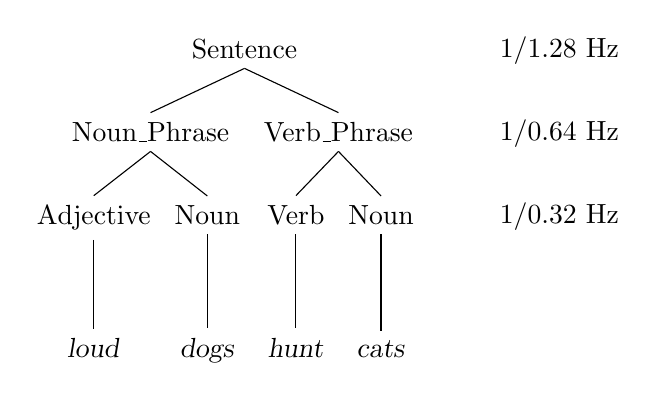
\begin{tikzpicture}
\tikzset{every tree node/.style={align=center,anchor=base}}
\tikzset{level 5+/.style={level distance=2\baselineskip}}
\tikzset{frontier/.style={distance from root=9\baselineskip}} \Tree
        [.Sentence [.Noun\_Phrase [.Adjective {\textsl{loud}} ] [.Noun
              {\textsl{dogs}} ] ] [.Verb\_Phrase [.Verb
              {\textsl{hunt}} ] [.Noun {\textsl{cats}} ] ] ] \node at
        (4,0.1) {1/1.28 Hz}; \node at (4,-0.95) {1/0.64 Hz}; \node at
        (4,-2.0) {1/0.32 Hz};
\end{tikzpicture}
\end{center}
\caption{Tree with frequencies \label{fig:freq_tree}}
\end{figure}

However, a considerable amount of behavioural data highlights the
significance of statistics during language comprehension. At the level
of word-statistics, word recognition times can largely be determined
by their frequency of occurrence in the language, word reading times
have been found to closely correlate with word probability and when an
ambiguous sentence has to be interpreted, the most probable
interpretation is most likely to be chosen (for review see
\cite{Jurafsky2002}). Additionally, both reading times and the
amplitude of neural responses are graded by the strength of
constraints imposed by prior context on possible sentence
continuations \cite{GibsonPearlmutter1998}. Language statistics must
therefore play a role in human language processing.

In a statistical description, the brain, in a Bayesian manner,
exploits the rich statistical structure of language to predict
possible identities for syllables, words and phrases and uses these
predictions to aid the identification of the actual linguistic
input. In this picture, the interpretation of language involves the
production, reevaluation and resolution of predictions, and grammar
has evolved out of a kind of \lq{}language game\rq{} where speakers
aid each other by propagating conventions about how words are
arranged, enriching the statistical structure of utterances and
syntactic categories are not psychologically real, but epiphenomenal
to a statistical-based response to linguistic stimuli.

In this context \cite{FrankYang2018} propose a computational model
that assumes no higher level of abstraction than a semantic clustering
of word representations. Their model represents each word as a
high-dimensional vector chosen so that the proximity structure of the
vectors matches the statistical relationship between the corresponding
words in a large language corpus. The frequency tagged experiment from
\cite{DingEtAl2016}, described above, were simulated and the model
generated power peaks at the same frequencies as those observed
experimentally. This suggests that the peaks could be generated using
only the lexical information within the word stimuli, without the need
for any knowledge of syntax.

Here human electroencephalography (EEG) is used to measure responses
to simple meaningful sentences in comparison to sentences with two
different manipulations; nonsense sentences which have been
deliberately chosen to have little sensible meaning, and ungrammatical
sentences, in which syntax has been destroyed by re-ordering the
words. The aim of this experiment is to help to distinguish between
the two competing explanations for the phrase- and sentence-level
phase locking observed in \cite{DingEtAl2016,DingEtAl2017}.

%this needs to be changed after Amelia changes the figure
We used EEG to record neural activity while subjects listened to
continuous streams of four single-syllable words that can combine to
form a sentence consisting of a noun phrase and a verb phrase. We
found that cortical responses become phase-locked to the frequencies
at which syllables, phrases and sentences are presented. A peak in the
ITPC value is observed at the sentential rate (1/1.28 Hz). This is
similar for sentences that are both grammatically correct and with
semantically sensible words and sentences that are ungrammatical in
terms of word order and contain semantically unrelated words. The peak
in the ITPC value at the rate of phrase presentation (2/1.28 Hz) is
maximal when sentences are both grammatical and make semantic
sense. This peak is reduced when either grammar or semantic sense
alone is lacking and is absent when sentences are both ungrammatical
and lack semantically-related words.


\section*{Methods}
\subsection*{Participants}

Eighteen right-handed, native English speakers (11 female, mean age 26
years (range 22 - 32 years)) participated in this study. All
participants gave written, informed consent prior to undertaking the
study and were paid £20. Participants were screened for dyslexia and hearing impairments. Ethical approval for our experimental procedures were obtained from the University of Bristol Faculty of
Science ethics board. All methods were performed in accordance with
the relevant guidelines and regulations.

\subsection*{Stimuli}

The experimental procedures were similar to those used in a recent EEG
study \cite{DingEtAl2017}. Listeners were played English sentences
composed of four single-syllable words. Each word was synthesised
independently using the MacinTalk Synthesizer (male voice Alex, in Mac
OS X 10.7.5). All of the synthesised words (226 - 365 ms) were
adjusted to 320 ms duration and volume normalised using the freely
available Praat software \cite{BoersmaWeenink2018}.

20 single-syllable words were chosen for each of the four word
categories: adjective, subject, verb, object. Words were selected if
they were synthesised clearly by the speech synthesizer and if they
could be easily categorised into a distinct word category.  This was
to avoid verbs, such as ``ride'', which can
also be used as nouns. Nouns were pluralised and all sentences were
played in the present tense.

Four conditions were created (see Table~\ref{\label{tab:conditions}): sensical and nonsensical
grammatical sentences (SG and NG) as well as two ungrammatical
conditions in which the words for sensical and nonsensical sentences
were re-ordered as verb, noun, noun, adjective: the SU and NU
conditions respectively. For the SG and NG grammatical sentences words
from the noun, adjective and verb categories were randomly selected
and ordered as
\begin{center}
  adjective, noun_1, verb, noun_2.
\end{center}
The resulting sentences were then independently ranked in terms of how
much sense they made by 290 online participants recruited through
Prolic Academic. Participants were presented with 110 pairs of
sentences, ten of these were an attention trap; participant were asked
to press `F' in response to sentences containing the word `fish' and
were punished with a time out if they made a mistake. For the
remaining 100 pairs they selected the sentence which `sounds more
normal in everyday speech'. Elo chess ranking \cite{Elo1978} was used
to derive individual scores for each sentence from the pairwise
comparisons. This established a ranking from sense to nonsense. The
top 20 sentences were chosen to form the sensical SG condition and the
bottom 20 were chosen to form the nonsensical NG conditions.  To
obtain the ungrammatical SU and NU conditions the words from the SG
and NG conditions respectively were re-ordered as
\begin{center}
verb, noun_1, noun_2, adjective.
\end{center}

\begin{table}
\begin{tabular}{l|ll}
&sensible&nonsense\\
\hline\\
grammatical&\textbf{SG}: huge trams scare boys&\textbf{NG}: bored mugs write beds\\
ungrammatical &\textbf{SU}: scare trams boys huge&\textbf{NU}: write mugs beds bored
\end{tabular}
\caption{A summary of the four conditions; the condition label used in the text is in
  bold, the sentence beside this gives an
  example.\label{tab:conditions}}
\end{table}

\subsection*{Experimental Procedures}

Each trial contained a sequence of thirteen four word sentences played back to back in a continuous stream. Each word was 320 ms long and trials lasted 16.64 seconds. In total, participants listened to 120 trials, with 30 trials for each of the four conditions. Blocks were made up of five trials from the same condition. Within each block, trials were presented to the participants one after the other with an 800 ms gap between trials. At the end of each block, participants were asked to rate the sentences on a scale of one
to five in terms of how much sense the sentences within the trials they had just heard made to them on average using a button press. Following the button press, the next block was played after a delay of 1200 ms. Blocks were presented in a random order and the order of the blocks was counterbalanced across participants. At the end of each block participants were given a ten second break, with a longer two minute break at the halfway point.

\subsection*{EEG Recording}

EEG signals were sampled at 1000 Hz from 32 Ag/AgCl electrodes fitted
on a standard electrode layout elasticised cap using a BrainAmp DC
amplifier (Brain Products GmbH). The EEG was recorded in DC mode,
using a low-pass filter of 1000 Hz (fifth-order Butterworth filter
with 30 dB/octave). FCz was used as a reference channel. The impedance
of the electrodes was kept below 5 kOhms. Recordings were analysed
offline using \texttt{Matlab} (Mathworks Inc.) and the
\texttt{Fieldtrip} toolbox \cite{FieldTrip}. Eyeblink artifacts were
removed using ICA. An independent component was removed if in its
topography the mean power over the most frontal four channels (Fp1,
Fp2, F7 and F8) was two times greater than the mean power over all
other channels, as in \citet{DingEtAl2017}. As our signals of interest
are in the low-frequency region, at 1/1.28 (sentences), 2/1.28
(phrases), and 4/1.28 Hz (syllables), the EEG signals were filtered
offline using a 25 Hz low-pass filter (sixth-order Butterworth
IIR). Data were re-referenced offline to a common average
reference. For each condition, individual trials (16.64s long) were
epoched. Upon sound onset there is a transient EEG response and so the
first four syllables (1.28 seconds) in each epoch were removed from
the analysis. This meant that the overall length of the analysed part
of each trial was 15.36 seconds, corresponding to 48 syllables x 0.32
s.


\subsection*{Data analysis}

The EEG signal for each trial was converted into the frequency
domain using the discrete Fourier transform with a frequency
resolution of 0.065 Hz, that is, 1/15.36 Hz. The complex-valued
Fourier coefficient of the trail $k$, $X_k(f)$, is then used to
calculate the inter-trial phase coherence .

The inter-trial phase coherence is defined as
\begin{equation}
\label{eq:itpc}
R(f)=\frac{1}{K}\left[\left(\sum_k{\cos{\theta_k(f)}}\right)^2+\left(\sum_k{\sin{\theta_k(f)}}\right)^2\right]
\end{equation}
where $\theta_k(f)$ is the phase angle of each complex-valued Fourier
coefficient $X_k(f)$ and $K$ is the total number of trials. As with
the evoked power, ITPC measures the time-locked response; because it
uses only the phase-angle rather than the whole response it does not
show the same $1/f$ noise that is present in the evoked power. As
such, it is a convenient measure of EEG response to a stimulus with
fixed frequency.

As in \cite{DingEtAl2016} a one-tailed paired t-test was used to test
whether the inter-trial phase coherence value in a given frequency bin
was significantly stronger than the average of the neighboring four
frequency bins, two bins on either side. This was applied to all
frequency bins below 5 Hz and a FDR correction for multiple
comparisons was applied.

A repeated measures, two-way ANOVA with a two (grammar: grammatical or
ungrammatical) by two (sense: sensical or nonsensical) factorial
design was performed to compare the main effects of grammar and
sensible meaning on the strength of the ITPC at target frequencies
across conditions. The TukeyHSD post-hoc test was used to compare the
strength of the ITPC responses at different frequencies of interest
(1/1.28 Hz, 2/1.28 Hz and 4/1.28 Hz) across each of the four
conditions for all participants. $p$ values of less than 0.05 indicate
a statistically significant result.


\section*{Results}

%Amelia to change this paragraph
Three significant peaks in the strength of the ITPC were observed in
the EEG response at the sentential (1/1.28 Hz), phrasal (2/1.28 Hz)
and syllabic (4/1.28 Hz) rates while subjects listened to four word
sentences (Fig.~\ref{Fig1}). These three peaks were significant in all
of the four sentence conditions except for the peak at the sentential
rate (1/1.28 Hz) in condition GS. In addition there is a
statistically significant peak at 3/1.28 Hz in three out of the four
conditions.

\begin{figure}[tbp]
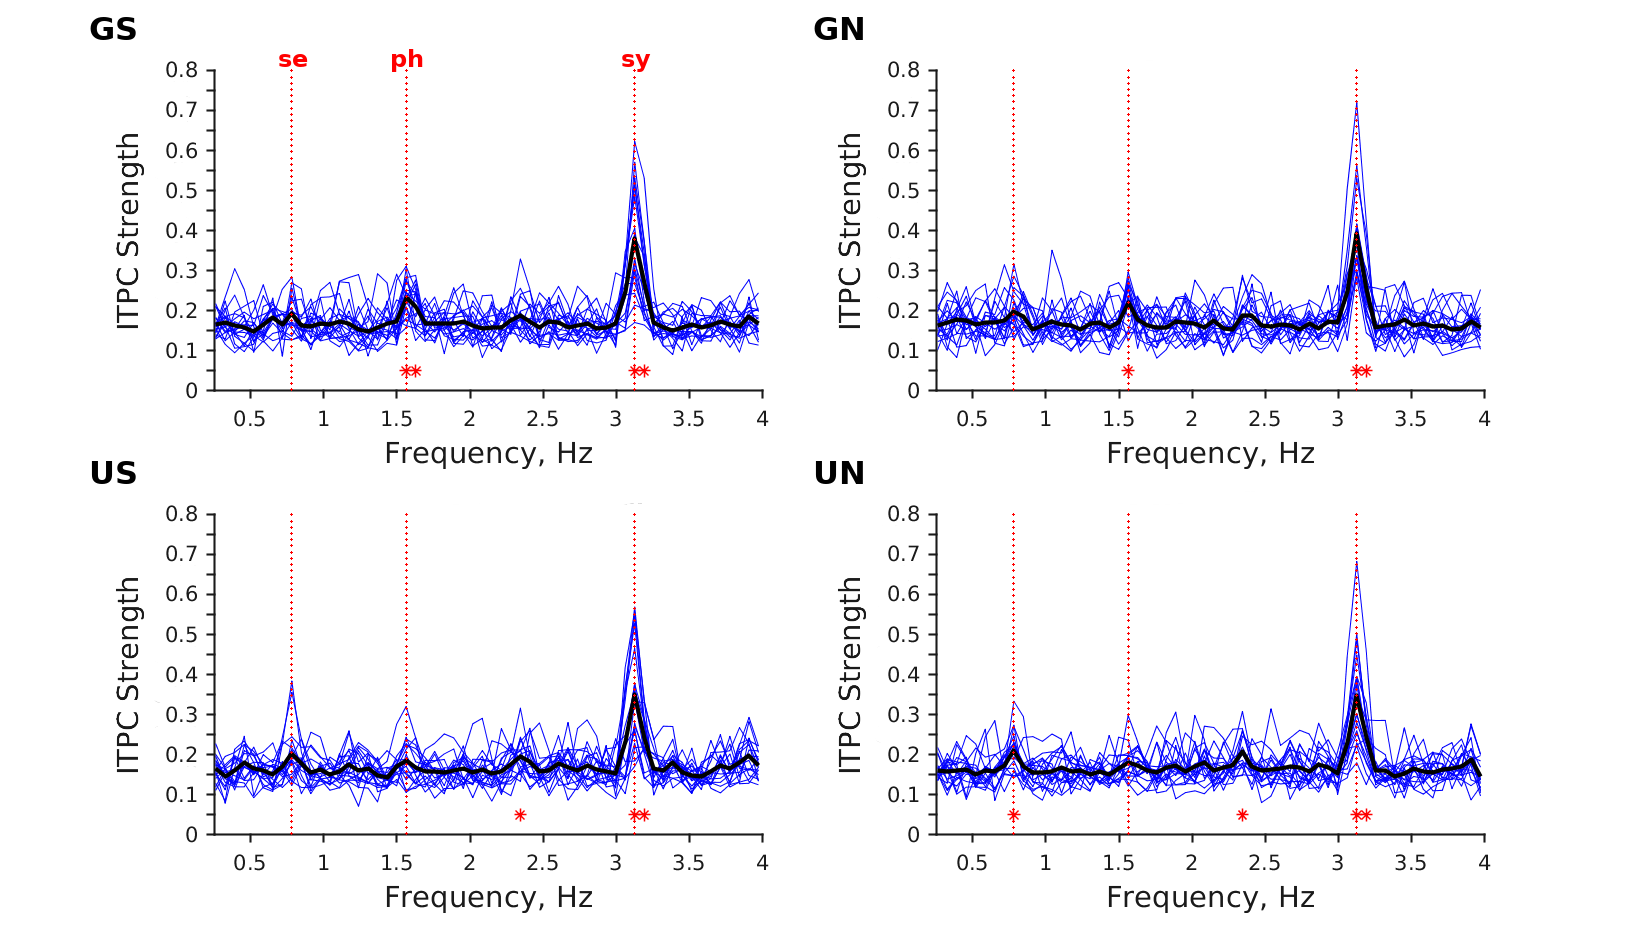
\includegraphics[width=\linewidth]{grand_average.png}
\caption{\textbf{The spectrum of inter trial phase coherence in the
    EEG response to sentences from each of the four conditions.} These
  figures show the grand average of ITPC over all participants and
  electrodes to each of the four condition; the grand average is in
  black, the blue lines are averages over all electrodes for the 18
  individual participants. Stars represent statistical significance of
  $p<0.05$.}
\label{Fig1}
\end{figure}

We analyzed whether there were significant main effects of grammar and
meaningful semantics on the strength of the inter-trial phase
coherence at each of the three frequencies of interest in the EEG
response (1/1.28 Hz, 2/1.28 Hz and 4/1.28 Hz),
Fig.~\ref{MainEffects}. A statistically significant effect of grammar
was observed at the syllabic rate, with a greater ITPC peak for
grammatically well-formed sentences ($F(1,17)=14.0673$, $n=18$ subjects,
$p=0.0016$, $\mu(\mathrm{G}) = 0.2402 \pm 0.1434$, $\mu(\mathrm{U}) =
0.2096 \pm 0.1381$; here, and elsewhere $\mu(\mathrm{C})$ is the mean of
condition C with the $\pm$ indicating the standard deviation). At the
rate of phrase presentation (2/1.28 Hz) there was a significant main
effect (Fig.~\ref{MainEffects}B) of both grammar and semantics: both
correct grammar and sensible semantics were associated with a
significantly greater peak in ITPC strength at the phrasal rate than
sentences with incorrect grammar or semantically unrelated words
(grammar: $F(1,17)=14.0673$, $n=18$ subjects $p=0.0016$, $\mu(\mathrm{G})=
0.2402 \pm 0.1434$, $\mu(\mathrm{U})= 0.2096 \pm 0.1381$; semantics:
 $F(1,17)=12.5283$, $n=18$ subjects, $p=0.0025$, $\mu(\mathrm{S}) = 0.0648
\pm 0.0328$, $\mu(\mathrm{N}) = 0.0459 \pm 0.0226$). No interaction
effects were observed ($p=0.7530$).

At the syllabic rate there was a significant main effect of grammar
(Fig.~\ref{MainEffects}C). The ITPC peak at the syllabic rate was
significantly greater when participants listened to grammatically
correct sentences compared to when the same participants listened to
grammatically incorrect sentences. No significant main
effect of semantics was observed (Fig.~\ref{MainEffects}C). At the
rate of sentence presentation no significant main effects on the
strength of ITPC were observed (Fig.~\ref{MainEffects}A).

\begin{figure}[tbp]
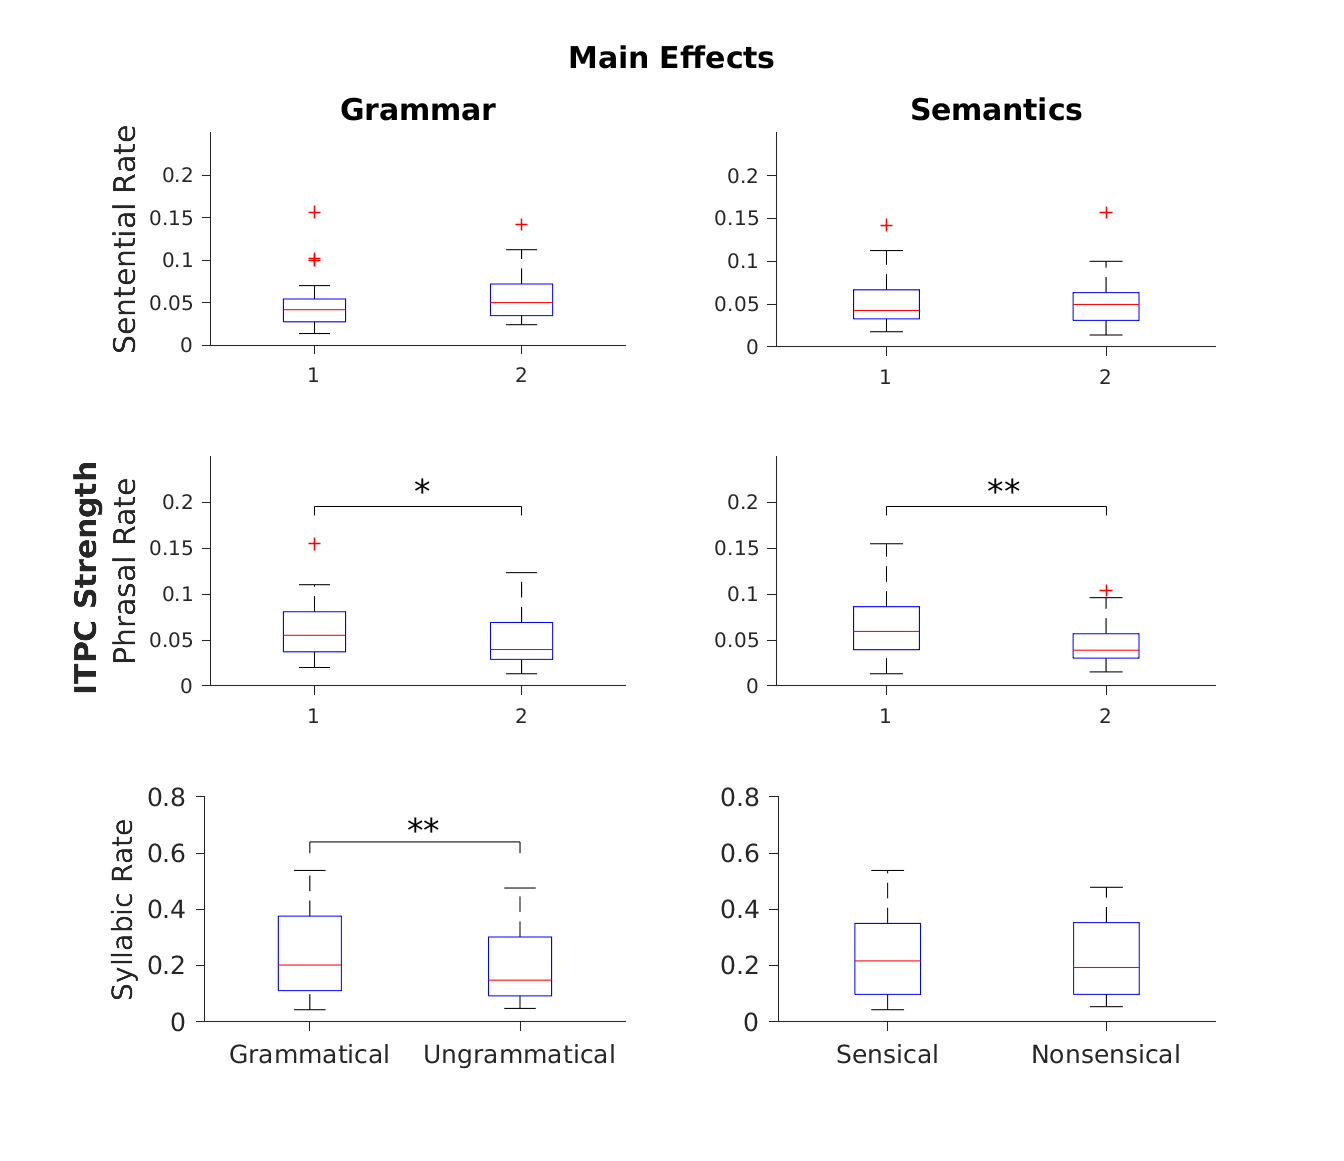
\includegraphics[width=\linewidth]{BoxPlots_main_effects.png}
\caption{\textbf{Main effects from the repeated measures 2-way ANOVA.}
  The main effects of grammar and sensible semantics on the strength
  of the ITPC at each of the three target frequencies of interest
  (sentence - 1/1.28 Hz, phrase - 2/1.28 Hz and syllalble - 4/1.28
  Hz). A statistically significant effect of grammar was observed at
  the syllabic rate, with a greater ITPC peak for grammatically
  well-formed sentences.  A main effect of grammar and semantics was
  also observed at the phrasal rate. No interactions between grammar
  and semantics are present.  *: $p<0.05$, **:$p<0.005$.  }
\label{MainEffects}
\end{figure}

The ITPC response at both the sentential and syllabic rate was similar
across all of the four conditions (Figure~\ref{ITPC_peaks}A,
~\ref{ITPC_peaks}C). We next compared the strength of the ITPC at the
rate of phrase presentation between each of the four experimental
conditions (Figure ~\ref{ITPC_peaks}B). The strength of the ITPC at
the phrasal rate is significantly greater in response to grammatically
well-formed, semantically sensible sentences in condition SG
($\mu(\mathrm{SG}) = 0.0712 +/- 0.0309$) compared to both condition NG
($p = 0.0328$, $\mu(\mathrm{NG}) = 0.0507 \pm 0.0242$) and condition
UN ($p = 0.0015$, $\mu(\mathrm{NU}) = 0.0411 \pm 0.0205$). No other
comparisons were significant.

\begin{figure}[tbp]
%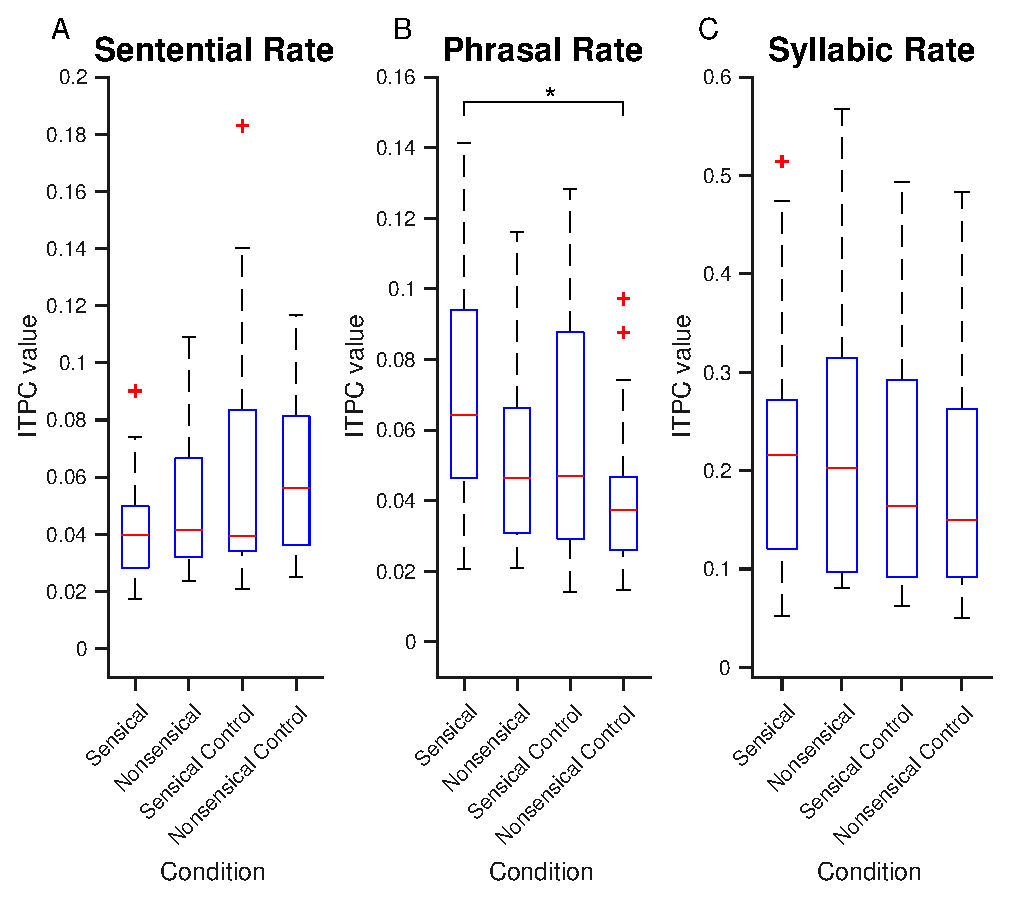
\includegraphics[width=\linewidth]{Figure3.eps}
\includegraphics[width=\linewidth]{ITPC_peaks_by_cond.png}
\caption{\textbf{Comparing ITPC values at frequencies of interest
    across conditions} Graphs showing average ITPC values at the
  sentential, phrasal and syllabic rates (\textbf{(A-C)}; 1/1.28 Hz,
  1/0.64 Hz, 1/0.32 Hz, respectively) for each of the four conditions
  tested. These are numbered along the $x$-axis as 1 - GS, 2 - GN, 3 -
  US and 4 - UN.  On the box plots the the central red line indicates
  the median ITPC value for each condition at each of the target
  frequencies \textbf{(A-C)}, the bottom and top edges of the box
  indicate the 25th and 75th percentiles of the ITPC values,
  respectively. The whiskers extend to the most extreme data points
  not considered outliers, and the outliers are plotted individually
  using the '+' symbol.  At the phrasal rate the SG condition is
  significantly higher than NG and NU. *:$p<0.05$, **:$p<0.005$,
  ***:$p<0.0005$. }
\label{ITPC_peaks}
\end{figure}

No effect of time was observed in the present study. The ITPC graphs
were similar when comparing trials that occurred at the beginning of
each experiment compared with trials that occurred later, and when
comparing the responses to sentences that were presented during the
first half of each trial with the last half of each trial. In cases
where conditions US and UN were presented to participants before
either conditions GS or GN, the peak in ITPC at the 1/1.28 Hz rate was
still evident. Therefore, the peak observed in ITPC at the sentential
rate to presentation in the ungrammatical conditions were not the
result of the expectancy of four word sentences given by the prior
presentation of sentences from the grammatical conditions.

\section*{Discussion}

The most basic effect was as predicted, is similar syllable-rate
effects in all four conditions.

Higher-level effects were less straigtforward. Eg the sentence peak
was missing in the GS condition contrary to previous research (DIng
2016, 2017, Makov et al 2017 - see
https://www.jneurosci.org/content/37/32/7772.abstract). The presence
of the sentence peak in the ungrammatical conditions agrees with Frank
& Yang's observation that statistical regularities at the level of
lexical category may be sufficient to induce a peak in the power
spectrum. Indeed the ungrammatical condition featured many lexical
category regularities at a 4-word cycle, e.g. both Adj and Verb
occurred every 4 words.

3- At the phrase rate, grammatical 2-word
phrases showed stronger ITPC than 2-word phrases in the ungrammatical
conditions (supporting the role of syntax in sentence
processing).

Interestingly, the ITPC for sensical conditions was higher than for
nonsensical condition at the phrase frequency (supporting the
importance of semantic information)

I would then conclude someho,
perhaps saying that the repetion of lexical category effect in 2 is
intereting and we explore in in (Burroughs et al Sci reports)

NB In
point 2 above I would not dwell onto why the sentence peak was missing
in SG condition beyond standard reasons like signal to noise etc and
the admittance that this is unexpected.

----

So, in
sum:

Given the lack of time and discussion of this among us in
light of the later Sci reports results I'd be as brief and as matter
of fact and non-speculating here as possible. 

ANd importantly I
would definitely delete the C&Chater para because the folloqing para
is not just consistent with them but in fact with ANY approach that
has a notion of a sentence.  I'd just leave the discussion of hte
points outlined above in this comment





We used EEG to record cortical activity in response to sentences
composed of four single-syllable words that can combine to form a noun
phrase and a verb phrase. We found that neural responses become
phase-locked to the frequencies at which syllables, phrases and
sentences are presented. This replicates the MEG and EEG studies
reported in \cite{DingEtAl2015,DingEtAl2017}. In this study we also
find both grammar and semantics effect the ITPC value at the phrase
rate.

In experimental conditions SU and NU, the four-word sentences are
ungrammatical and do not consitute well-formed sentences. The only
information that occurs at the sentential rate is therefore the
repetition of words that share a common syntactic category at the same
position across sentences. For example, a verb is repeated every four
words. In our data the peak at the senticial rate is weak and, in
fact, is only significant in the NU condition. The presence of an ITPC
peak at the sentential rate, even in the absence of syntactic
information or semantically related words, is indicative of language
processing at the word-level driven by syntactic category information
but not dependent on the hierachical processing of langauge based on
these categories.

This is supported by the fact that the occurrence of a particular word
does not usually allow for good prediction of the words that follow
it. As \cite{Pulvermuller2002}, states, it is likely that the regularities
governing word sequencies likely operate over lexical category. This
means that the presentation of a pronoun for example can predict, with
high probability, the later occurance of a compliment verb. For this
to be possible abstraction over word category is necessary. Our
results are inline with this theory.

In \cite{ChristiansenChater2016} it is argued that the key to
understanding the relationship between language and language
processing is to consider how serial processing of linguistic input
can occur despite the relatively small capacity of short term memory
and the long-range global dependencies present in language. Central to
their description is \lq{}chunk-and-pass\rq{}, the aggregating and
translating of sequential elements. This chunk-and-pass operation
occurs at multiple levels going from phonemes to words, words to
phrases, phrases to clauses and so on; the key idea is that in
linguistic processing, whenever possible, sets of sequential units are
translated into a unit with a more abstract representation. For the
\lq{}chunked\rq{} representation to be more compressed than the units
it replaces, there should be some dependency between these
units.

The findings presented here are consistient with this chunk-and-pass
description of language processing; in the SG condition the sentences
fall into natural chunks based on the syntax of the sentence, these
chunks are readily represented abstractly because the constituent
words for meaningful phrases and the process of chunking is aided by
the semantic regularity of the sentences. For the UN condition all
these elements are absent and the lack of a phrase peak in the ITPC
perhaps indicates that little chunking occurs at the phrase
level. From the perspective of chunk-and-pass it is perhaps surprising
that there is a phrasal peak for the SU condition, composed of
re-ordered sensical sentences; these sentences should lack any phrasal
structure. It would appear that the semantic relatedness of some
proximal words is sufficient for some chunking to occur at the phrase
rate. This suggests that semantics plays an important role in the
comprehension of spoken sentences.

It is possible that syntax and semantics can overlap to a certain
degree. \cite{Pulvermuller2002} suggests that the brain's responses to
words reflect both word semantics and lexical status;
\cite{KempsonEtAl2016} go further and suggest that syntax relies on
the incremental building of semantic representations. The experiment
reported here suggests that both correct syntactic and predictable
semantics need to occur together to generate a full brain response
during sentence comprehension. 


\bibliographystyle{clin}         
\bibliography{Sentences}

\end{document}

